\chapter{Struct, Union and Enum}

\section*{Introduction}
C++ provides \textbf{struct}, \textbf{union}, and \textbf{enum} as user-defined data types. They allow grouping of variables under one name for efficient data management.

\section{Structure (\texttt{struct})}

\subsection*{Definition}
A structure is a collection of variables (of different types) grouped together under a single name.

\subsection*{Syntax}
\begin{lstlisting}[caption=Syntax of struct]
struct StructName {
    dataType member1;
    dataType member2;
    ...
};
\end{lstlisting}

\subsection*{Example}
\begin{lstlisting}[caption=C++ Code using struct]
#include <iostream>
using namespace std;

struct Student {
    int roll;
    float marks;
    char grade;
};

int main() {
    Student s1 = {101, 95.5, 'A'};
    cout << "Roll: " << s1.roll << "\n";
    cout << "Marks: " << s1.marks << "\n";
    cout << "Grade: " << s1.grade << "\n";
    return 0;
}
\end{lstlisting}

\subsection*{Accessing Members with Pointer}
\begin{lstlisting}[caption=Accessing struct members using pointer]
Student s = {102, 88.4, 'B'};
Student *ptr = &s;
cout << ptr->roll << "\n";
cout << ptr->marks << "\n";
cout << ptr->grade << "\n";
\end{lstlisting}

\subsection*{Memory Representation}
\begin{center}
\begin{tabular}{|c|c|c|c|}
\hline
Member & Type & Size (Bytes) & Offset \\
\hline
roll & int & 4 & 0 \\
marks & float & 4 & 4 \\
grade & char & 1 & 8 (may pad to 12) \\
\hline
\end{tabular}
\end{center}

\subsection*{Diagram}
\begin{figure}[H]
\centering
\begin{tikzpicture}[node distance=0cm,outer sep=0pt]
\node[draw, minimum width=2cm, minimum height=1cm] (a) {roll};
\node[draw, minimum width=2cm, minimum height=1cm, right=of a] (b) {marks};
\node[draw, minimum width=2cm, minimum height=1cm, right=of b] (c) {grade};
\end{tikzpicture}
\caption{Memory layout of struct Student}
\end{figure}

\subsection*{Advantages}
\begin{itemize}
  \item Group heterogeneous data types.
  \item Enhances code clarity and reusability.
  \item Useful in data modeling (e.g., records, databases).
\end{itemize}

\section{Union (\texttt{union})}

\subsection*{Definition}
A union allows storing different data types in the same memory location. Only one member can hold a value at a time.

\subsection*{Syntax}
\begin{lstlisting}[caption=Syntax of union]
union UnionName {
    dataType member1;
    dataType member2;
    ...
};
\end{lstlisting}

\subsection*{Example}
\begin{lstlisting}[caption=C++ Code using union]
#include <iostream>
using namespace std;

union Data {
    int i;
    float f;
};

int main() {
    Data d;
    d.i = 10;
    cout << "Integer: " << d.i << "\n";

    d.f = 3.14;
    cout << "Float: " << d.f << "\n";

    // Now d.i is likely corrupted
    cout << "Integer after float: " << d.i << "\n";
    return 0;
}
\end{lstlisting}

\subsection*{Memory Representation}
\begin{center}
\begin{tabular}{|c|c|c|}
\hline
Member & Type & Size (Bytes) \\
\hline
i & int & 4 \\
f & float & 4 \\
\hline
\end{tabular}
\end{center}
\vspace{0.2cm}
\textbf{Total Memory:} Max of all members (4 bytes here)

\begin{figure}[H]
\centering
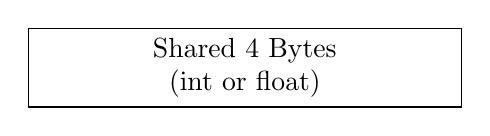
\begin{tikzpicture}
\draw (0,0) rectangle (5.5,1); % Wider box
\node at (2.75,0.5) {\parbox{5cm}{\centering Shared 4 Bytes\\(int or float)}};
\end{tikzpicture}
\caption{Union memory layout (shared memory)}
\end{figure}


\subsection*{Advantages}
\begin{itemize}
  \item Saves memory when only one member is used at a time.
  \item Useful in embedded systems and low-level programming.
\end{itemize}

\section{Enumeration (\texttt{enum})}

\subsection*{Definition}
An enum is a user-defined type consisting of a set of named integer constants.

\subsection*{Syntax}
\begin{lstlisting}[caption=Syntax of enum]
enum EnumName {
    CONSTANT1,
    CONSTANT2,
    ...
};
\end{lstlisting}

\subsection*{Example}
\begin{lstlisting}[caption=C++ Code using enum]
#include <iostream>
using namespace std;

enum Day {Mon, Tue, Wed, Thu, Fri, Sat, Sun};

int main() {
    Day d = Wed;
    cout << "Value of Wed: " << d << "\n";
    return 0;
}
\end{lstlisting}

\subsection*{Custom Values and Iteration}
\begin{lstlisting}[caption=Enum with custom values and loop]
enum Status {Pending=1, Approved=5, Rejected=10};

int main() {
    Status s = Approved;
    cout << "Status code: " << s << "\n";
    return 0;
}
\end{lstlisting}

\subsection*{Advantages}
\begin{itemize}
  \item Improves code readability.
  \item Restricts variable to valid set of values.
  \item Useful in state machines, switch cases.
\end{itemize}

\subsection*{Underlying Values}
\begin{verbatim}
By default: Mon = 0, Tue = 1, ..., Sun = 6
Custom: You can assign any value explicitly
\end{verbatim}

\begin{center}
\begin{tabular}{|c|c|}
\hline
Enum Constant & Value \\
\hline
Mon & 0 \\
Tue & 1 \\
Wed & 2 \\
Thu & 3 \\
Fri & 4 \\
Sat & 5 \\
Sun & 6 \\
\hline
\end{tabular}
\end{center}
